\chapter{Appendix}
\label{ch:appendix}

Gezien de lengte van het datascript werd het opgedeeld in vijf delen.

\begin{itemize}
	\label{app:datascript}
	\item \url{https://docs.google.com/document/d/1Sj3qtn06DYGMpT5jrAwTm1tS1ZqajHrA_-TzD4favOc/edit?usp=sharing}
	\item \url{https://docs.google.com/document/d/1Gd4PkCF84MkDOzdHtcRI5LAmG3ewnhuvQe2KQ8uzC18/edit?usp=sharing}
	\item \url{https://docs.google.com/document/d/1j8oia9qihzgOXcwtnLvaFb5y9yVSNfgHhOPb8Gyy_vw/edit?usp=sharing}
	\item \url{https://docs.google.com/document/d/18je4eFw3iFy1Whj-58CzKcTZy8eBgW-3OGzmM38ePkI/edit?usp=sharing}
	\item \url{https://docs.google.com/document/d/1m9Ubp4pNtj3WDhWAZwBSUTfB7cSPt2ZPgdFqfb9jgZ0/edit?usp=sharing}
\end{itemize}

In deel 1 worden de tabellen Like, LogType, Tile en TileType gecreëerd en opgevuld.
In deel 2 wordt de tabel Log gecreëerd en opgevuld.
In delen 3, 4 en 5 wordt de tabel Log verder opgevuld.

\begin{figure}
	\centering
	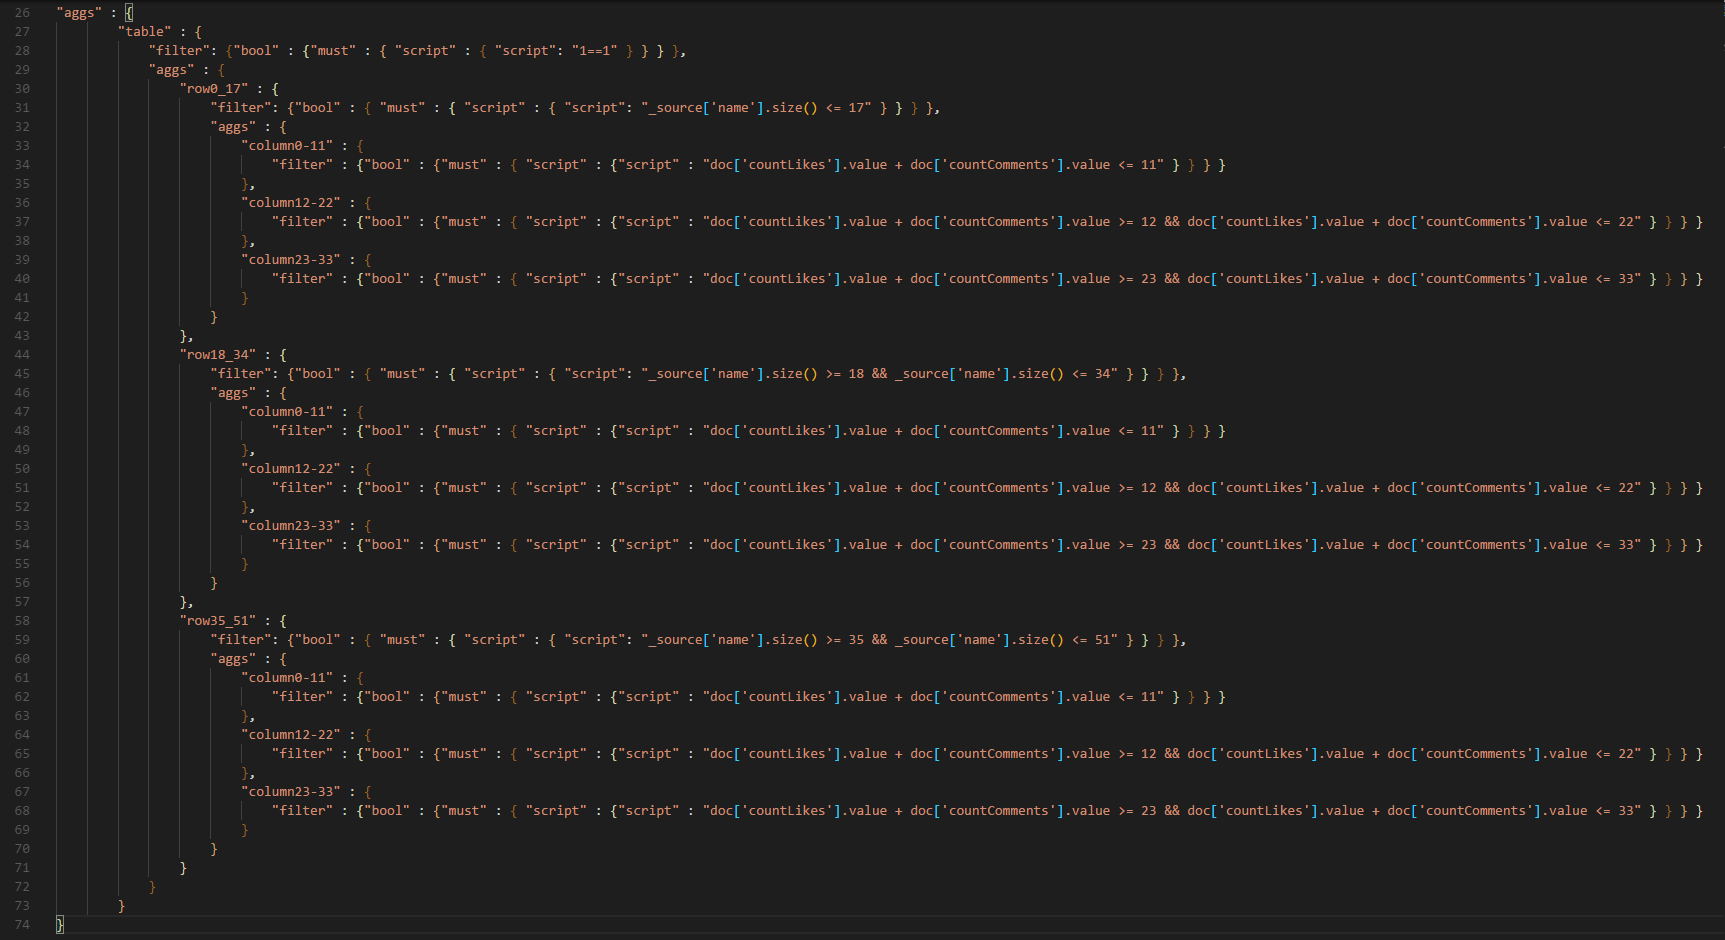
\includegraphics[width= 18cm]{script_table_wrong}
	\caption{Elasticsearch script voor het bekomen van de eerste kruistabel}
	\label{app:eersteKruistabel}
\end{figure}

\begin{figure}
	\centering
	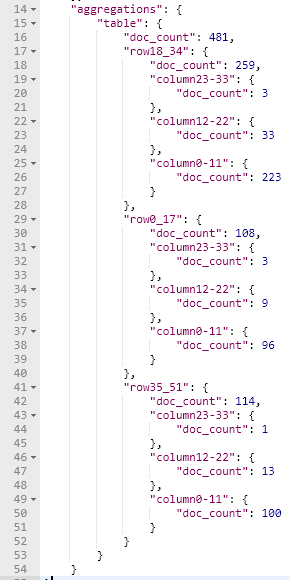
\includegraphics[width= 9cm]{script_table_wrong_result}
	\caption{Resultaat van het script voor het bekomen van de eerste kruistabel}
	\label{app:eersteKruistabelResult}
\end{figure}

\begin{figure}
	\centering
	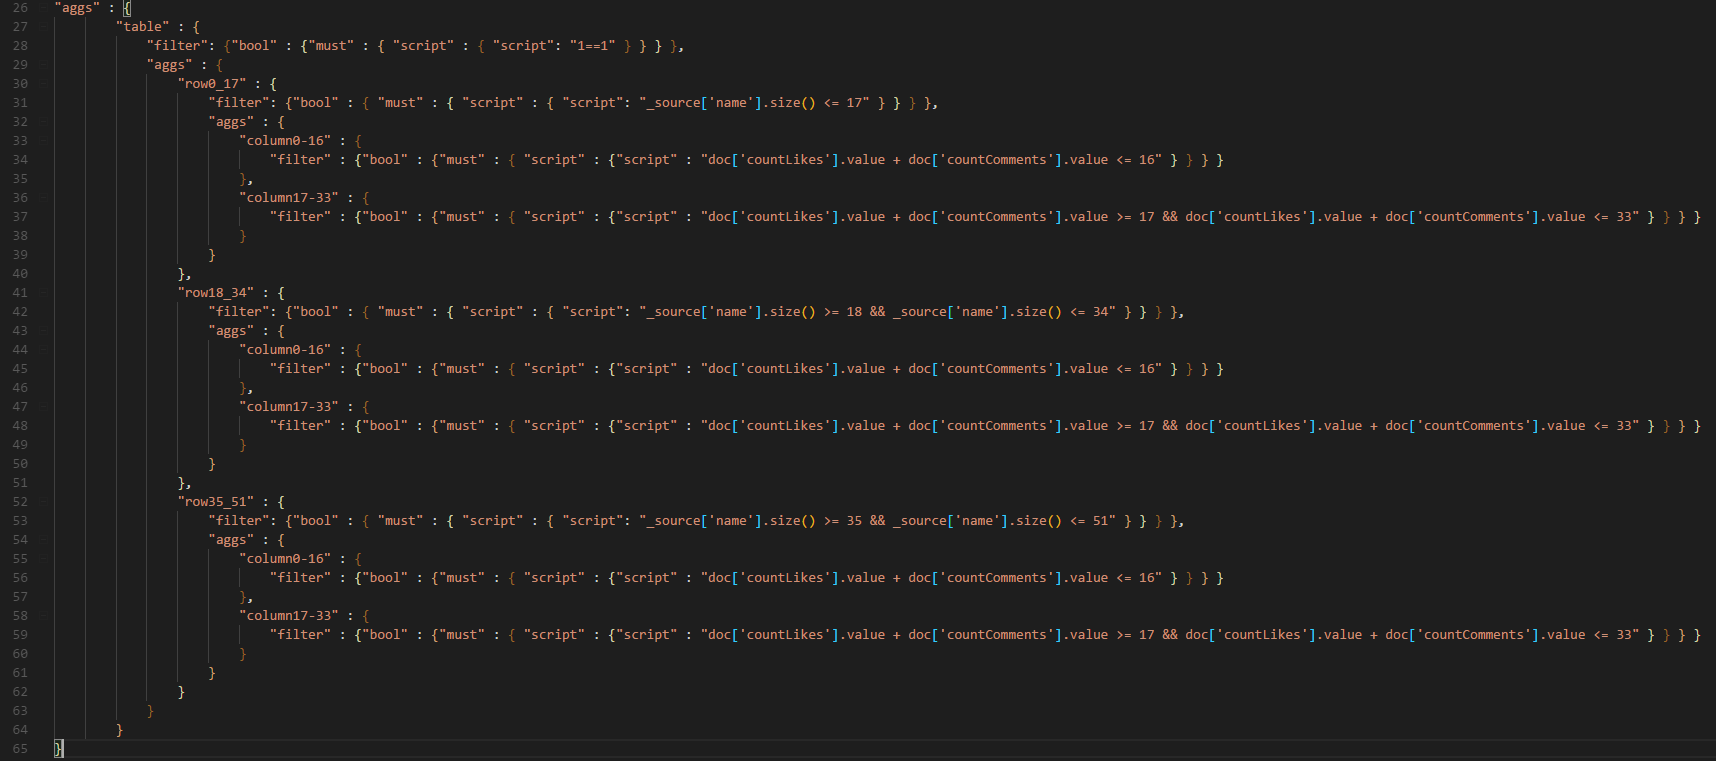
\includegraphics[width= 18cm]{script_table_correct}
	\caption{Elasticsearch script voor het bekomen van de tweede kruistabel}
	\label{app:tweedeKruistabel}
\end{figure}

\begin{figure}
	\centering
	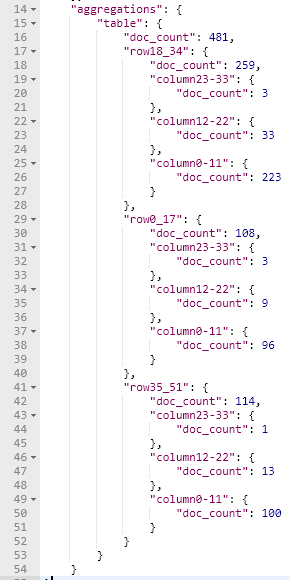
\includegraphics[width= 9cm]{script_table_wrong_result}
	\caption{Resultaat van het script voor het bekomen van de tweede kruistabel}
	\label{app:tweedeKruistabelResult}	
\end{figure}